\documentclass[11pt]{article}

% ---------- Packages ----------
\usepackage[utf8]{inputenc}
\usepackage[T1]{fontenc}
\usepackage[margin=1in]{geometry}
\usepackage{amsmath, amssymb}
\usepackage{booktabs}
\usepackage{array}
\usepackage{enumitem}
\usepackage{xcolor}
\usepackage{tikz}
\usetikzlibrary{shapes.geometric, arrows.meta, positioning, fit, backgrounds, calc}
\usepackage{listings}
\usepackage{hyperref}
\hypersetup{colorlinks=true, linkcolor=blue, urlcolor=blue}

% ---------- TikZ styles ----------
\tikzset{
  block/.style   = {rectangle, draw, rounded corners, align=center,
                     fill=blue!8, minimum height=1cm, minimum width=2.4cm,
                     inner sep=6pt},
  arrow/.style   = {-{Stealth[length=3mm]}, thick},
}

% ---------- Listings style ----------
\definecolor{codebg}{gray}{0.96}
\lstset{
  basicstyle=\ttfamily\small,
  backgroundcolor=\color{codebg},
  frame=single,
  rulecolor=\color{gray!40},
  breaklines=true,
  columns=fullflexible,
  keepspaces=true,
  showstringspaces=false,
  xleftmargin=6pt, xrightmargin=6pt,
  aboveskip=8pt, belowskip=8pt,
}

\title{\textbf{Phase 1 --- Transforms}\\[4pt]
\large Part B: homogeneous transforms in 2D}
\author{Robotics + AI Mentor Notes}
\date{\today}

\begin{document}
\maketitle

\begin{abstract}
\noindent Goal: pack \textbf{rotation + translation} into a single matrix so
combining frames becomes one clean multiplication. This is the exact tool ROS~2's
TF tree and every robot arm use to chain frames. You already built
\texttt{translate} and \texttt{rotate} (Part~A). Now we fuse them.
\end{abstract}

\tableofcontents
\bigskip
\hrule

% =====================================================================
\section{The problem with keeping rotation and translation separate}

A real camera is \textbf{both} rotated \emph{and} shifted relative to the robot
base. In Part~A you'd handle that in two steps: first \texttt{rotate}, then
\texttt{translate}. That works for one hop. But robots have \textbf{chains} of
frames:

\begin{center}
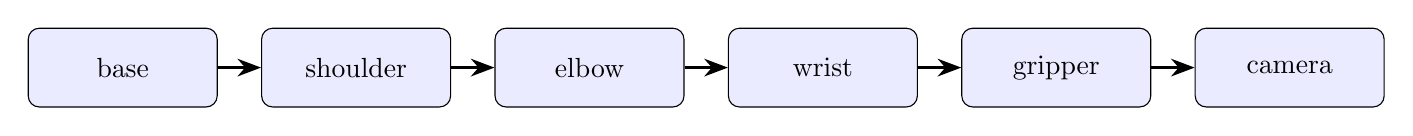
\begin{tikzpicture}[node distance=0.55cm]
  \node[block] (b) {base};
  \node[block, right=of b] (s) {shoulder};
  \node[block, right=of s] (e) {elbow};
  \node[block, right=of e] (w) {wrist};
  \node[block, right=of w] (g) {gripper};
  \node[block, right=of g] (c) {camera};
  \draw[arrow] (b) -- (s);
  \draw[arrow] (s) -- (e);
  \draw[arrow] (e) -- (w);
  \draw[arrow] (w) -- (g);
  \draw[arrow] (g) -- (c);
\end{tikzpicture}
\end{center}

Doing rotate-then-add at every link, by hand, is error-prone and ugly. We want a
single object per link that we can just \textbf{multiply together}. That object is
the \textbf{homogeneous transform matrix}.

% =====================================================================
\section{The trick: add a ``1'' to every point}

We glue an extra \texttt{1} onto each 2D point, making it a 3-vector:
\[
  \mathbf{p} = \begin{bmatrix} x \\ y \end{bmatrix}
  \;\longrightarrow\;
  \tilde{\mathbf{p}} = \begin{bmatrix} x \\ y \\ 1 \end{bmatrix}
\]
This is called \textbf{homogeneous coordinates}. That harmless-looking \texttt{1}
is what lets a single matrix multiply do \emph{both} rotation and translation at
once.

% =====================================================================
\section{The homogeneous transform matrix (2D)}

A rotation by $\theta$ \textbf{and} a translation $[t_x, t_y]$ combine into one
$3\times 3$ matrix:
\[
  T = \begin{bmatrix}
    \cos\theta & -\sin\theta & t_x \\
    \sin\theta & \cos\theta  & t_y \\
    0 & 0 & 1
  \end{bmatrix}
\]
\begin{itemize}[leftmargin=*]
  \item \textbf{Top-left $2\times 2$ block} $=$ the rotation matrix $R(\theta)$
  from Part~A.
  \item \textbf{Top-right column} $[t_x, t_y]$ $=$ the translation.
  \item \textbf{Bottom row} $[0,0,1]$ $=$ bookkeeping that keeps the math
  consistent.
\end{itemize}

Applying it to a homogeneous point does rotation \emph{then} translation in one
shot:
\[
  \tilde{\mathbf{p}}' = T\,\tilde{\mathbf{p}} =
  \begin{bmatrix}
    \cos\theta\,x - \sin\theta\,y + t_x \\
    \sin\theta\,x + \cos\theta\,y + t_y \\
    1
  \end{bmatrix}
\]
Then you \textbf{drop the last component} to get your 2D answer $[x', y']$.

\paragraph{Sanity checks (in your head):}
\begin{itemize}[leftmargin=*]
  \item $\theta=0,\ t=[1,0]$ applied to $[0.4,0.1]$ $\to$ $[1.4,0.1]$ (pure
  translation, matches Part~A).
  \item $\theta=90^\circ,\ t=[0,0]$ applied to $[1,0]$ $\to$ $[0,1]$ (pure
  rotation, matches Part~A).
  \item $\theta=90^\circ,\ t=[1,0]$ applied to $[1,0]$ $\to$ rotate
  $[1,0]{\to}[0,1]$, then add $[1,0]$ $\to$ $[1,1]$.
\end{itemize}

% =====================================================================
\section{Composing (chaining) frames $=$ matrix multiplication}

The real payoff: if $T_{A\leftarrow B}$ takes points from frame $B$ into $A$, and
$T_{B\leftarrow C}$ takes points from $C$ into $B$, then getting from \textbf{$C$
all the way to $A$} is just the matrix product:
\[
  T_{A\leftarrow C} = T_{A\leftarrow B}\; T_{B\leftarrow C}
\]
One multiply per link, chained down the arm. \textbf{This is why homogeneous
transforms exist.}

\begin{quote}
Order matters: the matrix on the \textbf{right} is applied to the point
\textbf{first}. $T_1 T_2 \mathbf{p}$ means ``do $T_2$, then $T_1$.''
\end{quote}

% =====================================================================
\section{Your task (implement + verify)}

Open \texttt{src/utils/homogeneous\_2d.py}. Implement:
\begin{enumerate}[leftmargin=*]
  \item \texttt{transform\_matrix(theta, tx, ty)} --- build the $3\times 3$ matrix
  above.
  \item \texttt{apply\_transform(T, point)} --- turn \texttt{point} into
  \texttt{[x, y, 1]}, multiply by \texttt{T}, return the 2D \texttt{[x', y']}
  (drop the trailing 1).
  \item \texttt{compose(T1, T2)} --- return the $3\times 3$ matrix product
  \texttt{T1 @ T2} (by hand, no numpy).
\end{enumerate}

Then run:
\begin{lstlisting}[language=bash]
cd ~/Music/projects_abbas/ROBOT_VLA
python3 src/utils/homogeneous_2d.py
\end{lstlisting}

\textbf{Expected output when correct:}
\begin{lstlisting}
[test] transform_matrix identity -> PASS
[test] pure translation          -> PASS
[test] pure rotation 90deg       -> PASS
[test] rotation + translation    -> PASS
[test] compose (chain frames)    -> PASS
All tests passed.
\end{lstlisting}

\textbf{If a test fails:} re-read the matrix in \S3, check row/column order, fix,
rerun. Report your output. Once green, we go to \textbf{Part C: 3D frames + the
ROS~2 TF tree.}

% =====================================================================
\section*{What's next (do NOT start yet)}
\addcontentsline{toc}{section}{What's next}
Part C: 3D homogeneous transforms ($4\times 4$) and how ROS~2 TF represents the
whole robot as a tree of these.

\end{document}
